\documentclass[journal]{IEEEtran}


\usepackage[T1]{fontenc} % hifenização (quebra de palavra)
\usepackage[utf8]{inputenc} % caracteres acentuados
\usepackage[brazil]{babel} % tradução inglês -> português; e. g., resumo ao invés de 
\usepackage[pdftex]{graphicx}
\usepackage{amsmath}
\usepackage{hyperref}

\hyphenation{op-tical net-works semi-conduc-tor}

\begin{document}

\title{Introdução ao Ray Tracing}

\author{ Lucas Araújo Pena \\ 
         13/0056162 }

% The paper headers
\markboth{Departamento de Ciência da Computação - 
Universidade de Brasília}%
{Shell \MakeLowercase{\textit{et al.}}: Introdução ao Ray Tracing}

\maketitle

% As a general rule, do not put math, special symbols or citations
% in the abstract or keywords.
\begin{abstract}
Lorem ipsum dolor sit amet, consectetur adipiscing elit. Donec id nisl eros. 
Phasellus eleifend nunc mi, nec rutrum purus lacinia sit amet. Vivamus eu 
tellus dui. Quisque fringilla nibh nec leo pretium eleifend. Nullam et mi in 
tortor laoreet viverra sit amet id ligula. Etiam vel mi a quam fringilla 
aliquam. Nulla facilisis pellentesque odio, sit amet iaculis arcu porta 
eget. Nunc ut tempor enim. In sit amet rhoncus metus. Sed euismod vulputate 
nulla non rutrum. Proin nisl est, blandit accumsan malesuada vel, pharetra a 
quam. Nam mollis nunc nisl, in ornare mi hendrerit id. Nullam posuere est 
ipsum, ac commodo neque ultrices at.
\end{abstract}


\begin{IEEEkeywords}
Computação Gráfica, Ray Tracing, Traçado de Raios, Path Tracing
\end{IEEEkeywords}

\section{Introdução}

\IEEEPARstart{O} Ray Tracing, uma técnica de renderização baseada na simulação do 
comportamento da luz, tem desempenhado um papel fundamental no avanço
dos gráficos por computador. Ao permitir a criação de imagens fotorrealistas, 
o Ray Tracing tem sido aplicado em várias áreas, como filmes de animação,
design de produtos e jogos digitais. Neste artigo, examinaremos a história 
do Ray Tracing, seus princípios teóricos e sua aplicação contemporânea, além 
de realizar um estudo de desempenho em um software de Ray Tracing. 

% Objetivo
O objetivo deste artigo é fornecer uma visão abrangente dessa técnica essencial
no campo da computação gráfica, discutir seu uso na atualidade, aprender como
funciona e como criar um Ray Tracer, e realizar uma análise de performance nesta
implementação, para que se possa ter uma ideia das complexidades envolvidas em
seu algoritmo.

%TODO 
% Achados da pesquisa

\section{Background}

Na computação gráfica, para que sejam gerados os mundos virtuais que todos conhecem,
é necessário que haja primeiro sua sintetização. Os métodos mais utilizados na atualidade
para renderizar uma cena virtual são a rasterização, o Ray Tracing e a mistura dos dois,
gerando uma renderização híbrida.

A rasterização é o método mais utilizado em aplicações que necessitam ser em tempo
real, como jogos eletrônicos e alguns tipos de simulações que precisam que haja
uma interação em tempo real, como um simulador de vôo para pilotos. A rasterização
é a conversão de um objeto em um ambiente virtual em pixeis para que seja mostrado
na tela. Este método foi otimizado para que gere imagens a partir de triângulos na
tela, por isso todo modelo 3D atualmente é uma malha de triângulos.
\cite{c12}

A rasterização é capaz de gerar resultados impressionantes, porém não alcança 
resultados fotorrealistas. Para se alcançar este tipo de resultado, o ray tracing
começou a ser utilizado.

\begin{figure}[!t]
\centering
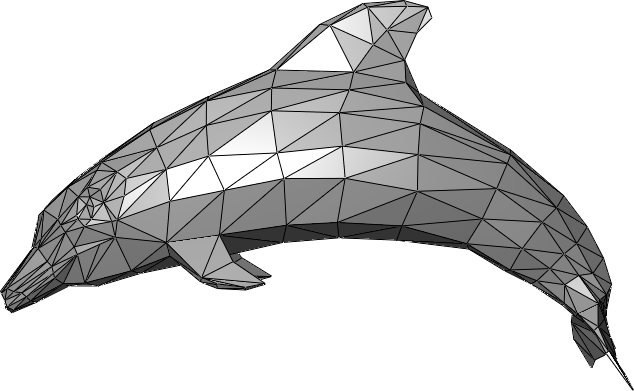
\includegraphics[width=2.5in]{media/mesh.png}
% where an .eps filename suffix will be assumed under latex, 
% and a .pdf suffix will be assumed for pdflatex; or what has been declared
% via \DeclareGraphicsExtensions.
\caption{Uma malha de polígonos.}
\label{fig_sim}
\end{figure}

O Ray Tracing, é uma técnica de renderização baseada na simulação do comportamento
da luz no mundo real. Os métodos mais utilizadas para a renderização atualmente
é a rasterização, onde a imagem é gerada a partir da varredura dos pixeis na
tela e calculando qual será o modelo a ser exibido e o Ray Tracing. Ao contrário da
abordagem utilizada pela rasterização, o Ray Tracing traça raios a partir da
câmera virtual da cena e simula a interação da luz nos objetos. Com este método,
é possível obter imagens foto realistas, com reflexos precisos, sombras suaves,
refrações e efeitos de iluminação complexos. 

A Rasterização processa as primitivas da cena de maneira diferente. Ela
utiliza um método onde as primitivas são dividias em triângulos, e a partir desta
divisão, 

Para diferenciar de maneira mais eficiente o Ray Tracing e a Rasterização, pode-se
resumidamente descrever o algoritmo dos dois. A Rasterização irá  para cada
primitiva, isto é, objeto em nosso mundo 3D, definir os pixeis na tela, enquanto
o Ray Tracing irá para cada pixel, definir a primitiva mais próxima. Considera-se
que estes dois métodos realizam uma operação inversa para a renderização.
\cite{c11}

É possível catalogar os principais métodos utilizando Ray Tracing em duas categorias: 
a \emph{Online} e a \emph{Offline.} O método \emph{Online} equivale dizer que é
maneira de renderização em tempo real. Este é o modelo mais desafiador, pois para
que uma simulação seja considerada tempo real, o Ray Tracing necessita do melhor
desempenho possível. Esta é uma das áreas mais estudadas do Ray Tracing, pois 
o Ray Tracing completo em tempo real é o tesouro que a indústria procura. Já a
metodologia do Ray Tracing \emph{Offline} é o modelo que utiliza a renderização
sem ser em tempo real, como animações e efeitos especiais para filmes. Nesta
abordagem, é possível a utilização do Ray Tracing completo e gerar a melhor imagem
possível que a técnica pode prover.Para que o  Ray Tracing \emph{Online}, chegue na
definição e complexidade do \emph{Offline}, será necessário um grande avanço na 
tecnologia dos dispositivos de processamento.
\cite{c11}

Na abordagem \emph{Online}, como é impraticável o uso do Ray Tracing completo, costuma-se
gerar uma parte da cena com o método de rasterização que é mais eficiente, e utiliza-se
o Ray Tracing para renderizar efeitos relacionados à iluminação e reflexos. Exemplos
de artefatos que o Ray Tracing pode gerar em conjunto com o a Rasterização são:
reflexos, sombras, oclusão de ambiente e iluminação global. Oclusão de ambiente
considera-se a sombra que cada objeto faz ao contato com outros objetos na cena,
e a Iluminação Global refere-se à iluminação gerada pelo Sol ou pelo céu, que
ilumina a cena por completo com uma fonte de luz que gera feixes de luz paralelos.
Na era em que este artigo está sendo escrito, não existem soluções satisfatórias
para Iluminação Global utilizando somente a Rasterização. É possível criar, porém
muitas vezes não atinge os padrões esperados para uma aplicação com uso do 
Ray Tracing.

Além desta classificação, o Ray Tracing pode ser classificado de acordo com o tipo
de algoritmo usado. Ray Tracing nada mais quer dizer que traçado de raios, ou seja,
traçar vetores dentro de uma cena 3D. Utilizando-se do método do Ray Tracing, também
temos o Path Tracing, que quer dizer Traçado de Caminho em português. A principal
diferença para o Ray Tracing convencional, é que o Path Tracing utiliza um modelo
de distribuição aleatória baseado nas características de Monte Carlo, e que ele gera
os raios a partir da câmera virtual até que cheguem em alguma fonte de luz. Esta é a 
principal abordagem utilizada pela indústria, pois gera a imagem ligeiramente
mais rápido e é possível utilizar outras técnicas em conjunto do Path Tracing,
que serão discutidas em outra seção.
\cite{c4}

O Ray Tracing também é utilizado para outros fins dentro de uma simulação além
da renderização. É possível utilizá-lo para simular áudio em VR, física, detecção
de colisão e para auxiliar a inteligência artificial. Estes métodos baseiam-se em
calcular o tamanho do traço que foi traçado para realizar os cálculos e as modificações
necessárias.
\cite{c10}

\subsection{Sua história}
É complicado definir um criador e uma data para este método. Porem, há vários
pesquisadores e artigos sobre o Ray Tracing que contribuíram significamente para
seu desenvolvimento e evolução. Um dos marcos para sua história foi o trabalho
de Arthur Appel em 1968 no artigo \emph{"Some Techniques for Shading Machine
Renderings of Solids"}. Neste trabalho, foi descrito os fundamentos do Ray Tracing
e foi apresentado técnicas para simular iluminação em objetos tridimensionais.
Outros nomes que aparecem em sua história são os de Turner Whitted, James Kajiya
e David Kirk. Uma destas contribuições que foi de bastante importância é a
Equação de Renderização, proposta por James em 1986. É uma equação que descreve
a iteração da luz em objetos tridimensionais, fornecendo um modelo matemático
para calcular a aparência de uma superfície e gerar imagens fotorrealistas.
A equação de renderização é definida desta maneira:

\[
L_o(\mathbf{p}, \mathbf{\omega_o}) = L_e(\mathbf{p}, \mathbf{\omega_o}) + \int_{\Omega} f(\mathbf{p}, \mathbf{\omega_i}, \mathbf{\omega_o}) L_i(\mathbf{p}, \mathbf{\omega_i}) (\mathbf{\omega_i} \cdot \mathbf{n}) d\mathbf{\omega_i}
\]

\vspace{10pt}
\begin{itemize}
  \item $L_o(p, \omega_o)$: Radiância de saída do ponto $p$ na direção $\omega_o$.
  \item $L_e(p, \omega_o)$: Radiância emitida pelo ponto $p$ na direção $\omega_o$.
  \item $f(p, \omega_i, \omega_o)$: Função de reflexão que descreve a interação da luz entre as direções $\omega_i$ e $\omega_o$ no ponto $p$.
  \item $L_i(p, \omega_i)$: Radiância incidente no ponto $p$ vinda da direção $\omega_i$.
  \item $\omega_i, \omega_o$: Direções incidente e de observação, respectivamente.
  \item $n$: Vetor normal à superfície no ponto $p$.
  \item $\Omega$: Hemisfério sólido que contém todas as direções de incidência.
\end{itemize}

Sua solução exata é bastante custosa, porém utilizando o Path Tracing, é possível
aproximá-la, graças ao modelo Monte Carlo de amostragem.

\subsection{Seu funcionamento}
O Ray Tracing mesmo não sendo trivial, é possível de se entender como funciona seu
algoritmo. Primeiro,
são traçados os chamados Raios Primários da câmera virtual, passando por cada pixel 
da imagem. São realizadas checagens para verificar se estes raios interceptaram algum 
objeto na cena.
Caso afirmativo, são gerados os Raios Secundários a partir do local de intersecção e
o ângulo que o raio atingiu o objeto. Quando isso ocorre, pode-se dizer que houve um
bounce, ou quique, em português. Através desta interação de raios com os objetos, é 
possível simular reflexões, refrações e sombras. Repete-se este procedimento até que
o critério de parada seja atingido. Normalmente, os critérios de parada são um número
máximo de bounces, ou se o raio não atingir nenhum objeto na cena. Neste caso, 
retorna-se a cor de fundo do ambiente, onde na maioria dos casos tem-se uma imagem
do horizonte, como uma Skybox, ou uma cor para representar o céu e o horizonte.

Esta técnica do Ray Tracing é interessante, pois nota-se que este algoritmo simula a física
de um feixe de luz no mundo real, porém na direção inversa. Por que não simular
como na vida real? Infelizmente, tentar simular todos os raios de luz saindo de uma fonte
de luz é extremamente custoso e não vale a pena em na maioria dos casos. Com este
algoritmo do Ray Tracing, pode-se simular somente os feixes de luz que atingem
a câmera virtual, poupando o processamento de feixes que não irão alterar nada
na cena. 


\subsection{Métodos de Iluminação e Modelos de Materiais}
Para que cada objeto possa reagir com a iluminação de maneira correta, cada objeto
possui uma propriedade que irá definir como será calculado sua textura. Estas propriedades
irão definir como irão interagir com o raio de luz, que são definidas para reflexão,
transparência e texturas. Para que seja definida a cor que o objeto terá, também se
determina qual será o modelo de reflexão usado. O mais utilizado na computação gráfica
é o modelo Phong.

O modelo Phong é utilizado para representar a iluminação em objetos, e é composto por
três componentes principais: ambiental, difusa e especular. O componente ambiental 
representa a luz ambiente que é refletida uniformemente em todas as direções pelo objeto.
É a cor base que ele terá independente das outras fontes de iluminação. O componente 
difuso descreve a reflexão difusa da luz incidente em uma superfície rugosa, que não
possui um reflexo com boa definição, por exemplo. A intensidade deste componente depende
do ângulo entre a direção da incidência da luz com a normal da superfície, ou seja, o 
vetor que sai da superfície em 90 graus. Em relação ao componente especular, este se 
trata da reflexão especular, que ocorre em superfícies polidas, como metais e espelhos.
A intensidade deste componente depende do ângulo entre a direção da luz refletida e a 
direção da câmera. Utiliza-se este componente para representar destaques brilhosos em
objetos.

\section{Seu uso na atualidade}
Atualmente, o Ray Tracing é bastante utilizado na media do entretenimento. Muito se 
fala do Ray Tracing em jogos no momento, mas ele também está presente no cinema, em
efeitos especiais ou filmes feitos inteiramente em animação.

\section{Avanços tecnológicos para o Ray Tracing}
Com a evolução das placas de vídeo e processadores, foi ficando cada vez mais
eficaz a renderização de simulações em 3D. Com o surgimento das placas de vídeo
dedicadas, a renderização que antes era feita pelo processador, agora poderia
ser feita pela placa de vídeo.

Para que o Ray Tracing pudesse ser implementado em simulações em tempo real,
como jogos eletrônicos, por exemplo, as fabricantes de placa de vídeo começaram
a desenvolver técnicas e chipes especiais focados em otimzar os cálculos do Ray 
Tracing. As técnicas mais utilitizadas para otimizar o desempenho e tornar possível
o uso de Path Tracing em tempo real incluem algoritmos de \emph{Upscaling}, que 
utilizam inteligência artificial para aumentar a resolução da imagem, onde a 
placa de vídeo renderiza o jogo em uma resolução menor e utiliza este algoritmo
para aumentar a sua resolução. Outra técnica utilizada e o \emph{Denoising},
onde utiliza-se o Path Tracing com poucos raios para gerar uma imagem incompleta
e através da inteligência artificial, gerar uma imagem completa.

\subsection{NVIDIA}
A NVIDIA foi a primeira empresa a criar uma placa de video com suporte nativo ao
Ray Tracing. A GeForce RTX 20 series, foram lançadas em setembro de 2018. Essa 
série de placas de vídeo apresentou uma tecnologia de ray tracing em tempo real 
chamada de NVIDIA RTX. A RTX 2080 Ti, que era a placa de vídeo mais pontente
desta série, possui 68 RT Cores, que são os núcleos dedicados ao Ray Tracing.
Além de um hardware dedicado, a NVIDIA também desenvolveu o DLSS, que significa
\emph{Deep Learning Super Sampling}, que utiliza inteligência artificial para
implementar o \emph{Upscaling}. Entretanto, como este era a primeira geração
de placas de video com componentes dedicados ao Ray Tracing, a maioria dos
jogos não conseguiam ter um bom desempenho com esta tecnologia funcionando,
principalmente sem o uso do DLSS. Em 2020, a NVIDIA lançou A GeForce 30
series, onde sua placa mais potente é a RTX 3090 Ti. Esta apresentou a
segunda geração de sua RT Cores, possuindo desta vez 84. Também foi apresentado
o DLSS 2.0, que teve um grande ganho em relação ao primeiro. Nesta etapa,
já era possível utilizar Ray Tracing em jogos utilizando o DLSS 2.0 e
adquirir um resultado minimamente satisfatório. Em 2022, foram lançadas as
NVIDA GeForce RTX 40 series. Até o momento de desenvolvimento deste artigo,
tem-se a RTX 4090 como a placa mais poderosa da NVIDIA. Esta placa possui
128 RT Cores, suporte ao novo DLSS 3.0 e à nova tecnologia desenvolvida
pela NVIDIA para melhorar o desempenho, que é o \emph{Frame Generation}.
Esta tecnologia cria frames novos entre dois frames, através da inteligência
artificial previamente treinada. 

Com a geração atual das placas da série 40 e todos estes outros recursos auxiliando
a renderização, como o DLSS 3.0 e o \emph{Frame Generation}, já é possível ter uma
experiência com Ray Tracing bastante satisfatória. Entretando, ainda não ha 
tecnologia o suficiente para que se possa ter um jogo ou simulação em
tempo real utilizando-se apenas o Ray Tracing. Os jogos que possuem esta
funcionalidade estão na categoria de renderização híbrida, utilizando a
rasterização para a maioria das cenas, porém deixando iluminação, sombras e/ou
reflexos para serem calculados pelo Ray Tracing.

\subsection{AMD}


\subsection{Intel}


\subsection{Outras}


\section{Definição Técnica}

\section{Como criar o seu Ray Tracer}

% Study Results
\section{Resultados de estudo}

\section{Conclusão}

\bibliographystyle{IEEEtran}
\bibliography{bibtex/bib/reference}

% that's all folks
\end{document}
